\chapter{Experiments}
\label{ch:experiments}


\section{The dataset}
A dataset was created to perform the experiments. In total there are 74 movies containing 20 different test subjects performing the complete sequence of 28 hand symbols. The movies where recorded with Sonic Gesture, with a resolution of 532x400 and a frame rate of 10. The test subjects where recorded while looking at a computer screen and asked to mimic the examples as in figure\ref{fig:hands_mirrored}, \ref{fig:hands_normal} and \ref{fig:hands_extra}. The movies with 12 test subjects where recorded with a simple (almost empty and smooth) background, 3 where recorded with a complex background and 6 where recorded with the same complex background but also with a poster with skinlike colors.

\begin{table}
\centering
\begin{tabular}{llll}
\hline\hline
	Test Subject & Movies & Background & Notes \\
\hline
	Anne     & 5 & Simple & None \\
	Arjan    & 5 & Simple & None \\
	Gijs     & 5 & Simple & None \\
	Ivo      & 5 & Simple & None \\
	Jasper 1 & 5 & Simple & None \\
	Peter    & 5 & Simple & None \\
	Hanne    & 5 & Simple & None \\
	Jasper 2 & 3 & Simple & None \\
	Ork      & 3 & Simple & None \\
	Roberto  & 3 & Simple & None \\
	Xiaong   & 3 & Simple & None \\
	\hline			
	Gosia    & 3 & Complex & None \\
	Hamdi    & 3 & Complex & None \\
	Michael  & 3 & Complex & None \\
	Sil      & 3 & Complex + skin-like colors & None \\
	Victoria & 3 & Complex + skin-like colors & None \\
	Chu      & 3 & Complex + skin-like colors & problem with brick wall \\
	\hline	
	Bas      & 3 & Complex + skin-like colors & None \\
	Koen     & 3 & Complex + skin-like colors & None \\
	Stratos  & 3 & Complex + skin-like colors & problems with white wall \\
\hline
\end{tabular}
\caption{Dataset details}
\end{table}

The dataset is manually labeled. For every sequence of frames where a hand pose is performed a frame number is labeled where the pose resembles the example the most. Figure\ref{fig:gijs5} is an example of the labeled frames.

Usually the 12 Curwen solfege hand symbols are performed in front of the torso as shown in Figure~\ref{fig:hands_normal}. To increase the number of hand poses to be recogniced, all 12 Curwen are also performed mirrored next to the body of the recorded subject, see Figure~\ref{fig:hands_mirrored}. Additionally four extra hand symbols have been added that are not part of the Curwen sequence, see Figure~\ref{fig:hands_extra}. These last four symbols are performed next to the head.

\section{Evaluation}


\section{Implementation}
OpenCV, QT, CMake, Liblo, open source, website

\section{Results}

\subsection{part I}
For the number of neighbours for KNN a small number of tests where run, and a choice was made for a value of 3. higher values untill around 10 yield similar performance, depending on the test. Lower than 3 or higher than 10 will decrease performance.

When PCA was used the smallest eigenvectors where removed so 95\% of the original variance was kept.

For SVM the radial basis function (RBF) kernel is used, since the libsvm documentation states that is a good kernel to use that usually gives good performance. The $c$ and $\gamma$ values for SVM where found by an extensive grid search on the 'per person' tests with only the simple movies performed on a small cluster in the ranges $2.^(-3:2:15)$ for $c$ and $2.^(-15:2:3)$ for $\gamma$. The most optimal values are $\gamma$ = 0.03125. With this $\gamma$ changing the value for $c$ didn't have much effect on the performance, so a value of 64 was choosen.

Doing PCA and removing eigenvectors untill 0.95 variance on the simple data set will reduce to  594 dimensions (from 3780);
complex + simple: 688
complex:  283
full: 749


\begin{table}
\centering
\begin{tabular}{lrr}
\hline\hline
Classifier 				&  	Full scale	& Major scale	\\
\hline
KNN3 		&  	84.27\%		& 90.21\%		\\
PCA, KNN3 	& 	83.67\%		& 89.70\%		\\
PCA, SVM RBF ($c=1$ $\gamma=\frac{1}{|features|}$)	& 	76.78\%		& 84.38\%		\\
SVM RBF ($c=2^6$ $\gamma=2^{-5}$) & 86.02\% & 90.88\% \\
PCA, SVM RBF ($c=2^6$ $\gamma=2^{-5}$) &  86.85\% & 91.85\% \\
SVM $\chi^2$ & 87.92\% 		& 91.58\% \\
\hline
\end{tabular}
\caption{k-fold per film using simple dataset only}
\end{table}


\begin{table}
\centering
\begin{tabular}{llrr}
\hline\hline
Dataset & Classifier 				&  	Full scale	& Major scale	\\
\hline
simple set	& KNN3	& 72.93\%, & 82.63\%	\\
simple set	& PCA, SVM RBF ($c=2^6$ $\gamma=2^{-5}$) & 79.71\%, & 86.70\%	\\
full set	& KNN3 & 66.98\%, & 76.32\%	\\
full set	& PCA, KNN3 & 65.31\%, & 76.00\%	\\
full set	& PCA, SVM RBF ($c=1$ $\gamma=\frac{1}{|features|}$) & 64.05\%, & 74.42\%	\\
full set	& PCA, SVM RBF ($c=2^6$ $\gamma=2^{-5}$)& 73.38\%, & 81.44\%	\\
full set    & SVM $\chi^2$ &  71.83\% &80.07\% \\
\hline
\end{tabular}
\caption{k-fold per person}
\end{table}


\begin{table}
\centering
\begin{tabular}{lcc}
\hline\hline
Classifier 				&  	Full scale	&	Major scale	\\
\hline
KNN3					&	58.57\% 	&	72.78\%	\\
PCA, KNN3 				&	57.62\% 	&	72.17\%	\\
PCA, SVM RBF ($c=1$ $\gamma=\frac{1}{|features|}$)	& 55.48\%	&	68.25\%	\\
PCA, SVM RBF ($c=2^6$ $\gamma=2^{-5}$)				& 62.14\%	&	73.39\%	\\
SVM $\chi^2$ 			&	63.81\%		&	74.71\%	\\
\hline
\end{tabular}
\caption{simple as trainset, complex as test}
\end{table}



\begin{table}
\centering
\begin{tabular}{
|@{\hspace{0.4ex}}r@{\hspace{0.4ex}}@{\hspace{0.4ex}}r@{\hspace{0.4ex}}
|@{\hspace{0.4ex}}r@{\hspace{0.4ex}}@{\hspace{0.4ex}}r@{\hspace{0.4ex}}
|@{\hspace{0.4ex}}r@{\hspace{0.4ex}}
|@{\hspace{0.4ex}}r@{\hspace{0.4ex}}@{\hspace{0.4ex}}r@{\hspace{0.4ex}}
|@{\hspace{0.4ex}}r@{\hspace{0.4ex}}@{\hspace{0.4ex}}r@{\hspace{0.4ex}}
|@{\hspace{0.4ex}}r@{\hspace{0.4ex}}@{\hspace{0.4ex}}r@{\hspace{0.4ex}}
|@{\hspace{0.4ex}}r@{\hspace{0.4ex}}
|@{\hspace{0.4ex}}r@{\hspace{0.4ex}}@{\hspace{0.4ex}}r@{\hspace{0.4ex}}
|@{\hspace{0.4ex}}r@{\hspace{0.4ex}}@{\hspace{0.4ex}}r@{\hspace{0.4ex}}
|@{\hspace{0.4ex}}r@{\hspace{0.4ex}}
|@{\hspace{0.4ex}}r@{\hspace{0.4ex}}@{\hspace{0.4ex}}r@{\hspace{0.4ex}}
|@{\hspace{0.4ex}}r@{\hspace{0.4ex}}@{\hspace{0.4ex}}r@{\hspace{0.4ex}}
|@{\hspace{0.4ex}}r@{\hspace{0.4ex}}@{\hspace{0.4ex}}r@{\hspace{0.4ex}}
|@{\hspace{0.4ex}}r@{\hspace{0.4ex}}
|@{\hspace{0.4ex}}r@{\hspace{0.4ex}}@{\hspace{0.4ex}}r@{\hspace{0.4ex}}@{\hspace{0.4ex}}r@{\hspace{0.4ex}}@{\hspace{0.4ex}}r@{\hspace{0.4ex}}
|}

\hline
31 & 5 & 1 & 0 & 0 & 0 & 0 & 1 & 0 & 0 & 0 & 0 & 0 & 0 & 0 & 0 & 0 & 0 & 1 & 0 & 0 & 0 & 0 & 0 & 0 & 0 & 0 & 3 \\
6 & 35 & 0 & 0 & 0 & 0 & 0 & 1 & 0 & 0 & 0 & 0 & 0 & 0 & 0 & 0 & 0 & 0 & 0 & 0 & 0 & 0 & 0 & 0 & 0 & 0 & 0 & 0 \\
\hline
0 & 0 & 33 & 3 & 1 & 0 & 1 & 0 & 0 & 1 & 0 & 1 & 0 & 0 & 0 & 0 & 0 & 0 & 0 & 0 & 0 & 0 & 0 & 0 & 0 & 0 & 0 & 2 \\
0 & 0 & 5 & 31 & 3 & 0 & 0 & 0 & 0 & 0 & 0 & 1 & 0 & 0 & 0 & 0 & 0 & 0 & 0 & 0 & 0 & 0 & 0 & 0 & 0 & 0 & 0 & 2 \\
\hline
0 & 0 & 1 & 1 & 27 & 0 & 6 & 0 & 1 & 0 & 0 & 1 & 0 & 0 & 0 & 0 & 1 & 0 & 1 & 0 & 0 & 0 & 0 & 0 & 0 & 0 & 0 & 3 \\
\hline
0 & 0 & 0 & 0 & 0 & 37 & 0 & 0 & 0 & 0 & 0 & 0 & 0 & 0 & 1 & 1 & 0 & 0 & 0 & 1 & 0 & 0 & 0 & 0 & 0 & 2 & 0 & 0 \\
0 & 0 & 0 & 1 & 2 & 0 & 30 & 2 & 0 & 1 & 0 & 0 & 0 & 0 & 0 & 1 & 0 & 1 & 0 & 1 & 0 & 1 & 0 & 0 & 0 & 0 & 0 & 2 \\
\hline
0 & 0 & 0 & 0 & 0 & 0 & 0 & 40 & 1 & 0 & 0 & 0 & 0 & 0 & 0 & 0 & 1 & 0 & 0 & 0 & 0 & 0 & 0 & 0 & 0 & 0 & 0 & 0 \\
0 & 0 & 0 & 0 & 0 & 0 & 0 & 6 & 36 & 0 & 0 & 0 & 0 & 0 & 0 & 0 & 0 & 0 & 0 & 0 & 0 & 0 & 0 & 0 & 0 & 0 & 0 & 0 \\
\hline
0 & 0 & 3 & 0 & 0 & 0 & 0 & 0 & 0 & 31 & 1 & 6 & 0 & 0 & 0 & 0 & 0 & 0 & 0 & 0 & 0 & 0 & 0 & 0 & 0 & 0 & 0 & 1 \\
0 & 0 & 0 & 1 & 0 & 0 & 0 & 0 & 0 & 4 & 34 & 0 & 0 & 0 & 0 & 0 & 0 & 1 & 1 & 0 & 0 & 0 & 0 & 0 & 0 & 0 & 0 & 1 \\
\hline
0 & 0 & 0 & 1 & 1 & 0 & 0 & 0 & 0 & 1 & 0 & 38 & 0 & 0 & 0 & 0 & 0 & 0 & 0 & 0 & 0 & 0 & 0 & 0 & 0 & 0 & 0 & 1 \\
\hline
0 & 0 & 0 & 0 & 0 & 0 & 0 & 0 & 0 & 0 & 0 & 0 & 41 & 0 & 0 & 0 & 0 & 0 & 0 & 1 & 0 & 0 & 0 & 0 & 0 & 0 & 0 & 0 \\
0 & 0 & 0 & 0 & 0 & 0 & 0 & 0 & 0 & 0 & 0 & 0 & 3 & 38 & 0 & 0 & 0 & 0 & 0 & 0 & 1 & 0 & 0 & 0 & 0 & 0 & 0 & 0 \\
\hline
0 & 0 & 0 & 0 & 0 & 0 & 0 & 0 & 0 & 0 & 0 & 0 & 0 & 0 & 36 & 4 & 1 & 0 & 0 & 0 & 0 & 0 & 0 & 0 & 0 & 0 & 0 & 1 \\
0 & 0 & 0 & 0 & 0 & 0 & 0 & 0 & 0 & 0 & 0 & 0 & 0 & 0 & 4 & 34 & 1 & 0 & 0 & 0 & 0 & 0 & 3 & 0 & 0 & 0 & 0 & 0 \\
\hline
0 & 0 & 0 & 0 & 3 & 0 & 0 & 0 & 0 & 0 & 0 & 1 & 0 & 0 & 3 & 0 & 29 & 1 & 1 & 1 & 0 & 1 & 0 & 0 & 0 & 0 & 0 & 2 \\
\hline
0 & 0 & 0 & 0 & 0 & 0 & 0 & 0 & 0 & 0 & 0 & 0 & 0 & 0 & 0 & 0 & 0 & 40 & 0 & 0 & 0 & 1 & 0 & 0 & 0 & 0 & 0 & 1 \\
0 & 0 & 0 & 0 & 0 & 0 & 0 & 0 & 0 & 0 & 0 & 0 & 0 & 0 & 0 & 0 & 0 & 0 & 37 & 0 & 1 & 0 & 0 & 2 & 0 & 0 & 0 & 2 \\
\hline
0 & 0 & 0 & 0 & 0 & 0 & 0 & 0 & 0 & 0 & 0 & 0 & 0 & 0 & 0 & 0 & 0 & 0 & 0 & 41 & 1 & 0 & 0 & 0 & 0 & 0 & 0 & 0 \\
0 & 0 & 0 & 0 & 0 & 0 & 0 & 0 & 0 & 0 & 0 & 0 & 0 & 0 & 0 & 0 & 0 & 0 & 0 & 6 & 36 & 0 & 0 & 0 & 0 & 0 & 0 & 0 \\
\hline
0 & 0 & 0 & 0 & 1 & 0 & 1 & 0 & 0 & 0 & 0 & 0 & 0 & 0 & 2 & 3 & 1 & 1 & 0 & 0 & 0 & 28 & 4 & 0 & 0 & 0 & 0 & 1 \\
0 & 0 & 0 & 0 & 0 & 0 & 0 & 0 & 0 & 0 & 0 & 0 & 0 & 0 & 1 & 5 & 0 & 0 & 0 & 0 & 0 & 2 & 33 & 0 & 0 & 0 & 0 & 1 \\
\hline
0 & 0 & 0 & 0 & 0 & 0 & 0 & 0 & 0 & 0 & 0 & 0 & 0 & 0 & 2 & 1 & 0 & 0 & 1 & 0 & 0 & 2 & 0 & 34 & 0 & 0 & 1 & 1 \\
\hline
0 & 0 & 0 & 0 & 0 & 0 & 0 & 0 & 0 & 0 & 0 & 0 & 0 & 0 & 0 & 0 & 0 & 0 & 0 & 0 & 0 & 0 & 0 & 0 & 41 & 0 & 1 & 0 \\
0 & 0 & 0 & 0 & 0 & 0 & 0 & 0 & 0 & 0 & 0 & 0 & 0 & 0 & 0 & 0 & 0 & 0 & 0 & 0 & 0 & 0 & 0 & 0 & 0 & 41 & 0 & 1 \\
0 & 0 & 0 & 0 & 0 & 0 & 0 & 0 & 0 & 0 & 0 & 0 & 0 & 0 & 1 & 0 & 0 & 0 & 0 & 0 & 0 & 0 & 0 & 0 & 0 & 0 & 41 & 0 \\
1 & 0 & 0 & 0 & 0 & 0 & 0 & 0 & 0 & 0 & 0 & 0 & 0 & 0 & 0 & 0 & 1 & 1 & 1 & 0 & 0 & 0 & 0 & 0 & 0 & 0 & 0 & 38 \\
\hline
\end{tabular}
\caption{confusion matrix fro simple set, KNN3, per film}
\end{table}

\subsection{Part II}

For this set of experiments the Damerau–Levenshtein distance of a sequence of generated labels to the ground truth is calculated.


\section{Discussion}
As you can see there is a big difference in performance



\section{Images}

\renewcommand{\thesubfigure}{\thefigure.\roman{subfigure}}
\begin{figure}[htbp]
\begin{center}
\subfloat[Do]{\label{fig:hand_0}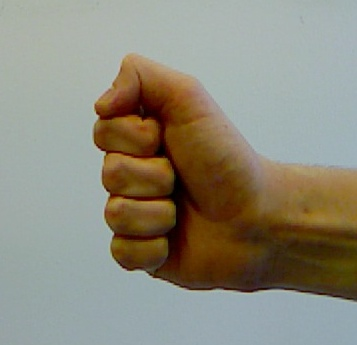
\includegraphics[width=0.2\linewidth,height=0.15\linewidth]{figures/examples/0.jpg}}
\hspace{0.03\linewidth}
\subfloat[Di]{\label{fig:hand_1}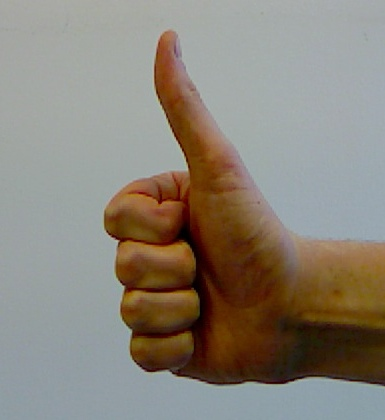
\includegraphics[width=0.2\linewidth,height=0.15\linewidth]{figures/examples/1.jpg}}
\hspace{0.03\linewidth}
\subfloat[Re]{\label{fig:hand_2}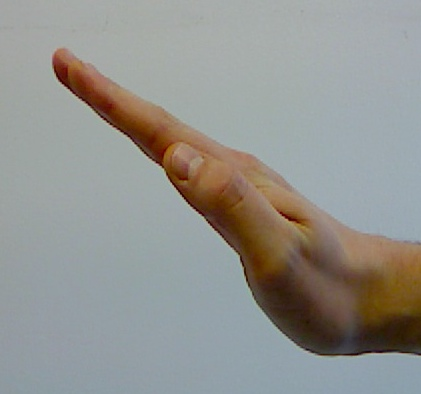
\includegraphics[width=0.2\linewidth,height=0.15\linewidth]{figures/examples/2.jpg}}
\hspace{0.03\linewidth}
\subfloat[Ri]{\label{fig:hand_3}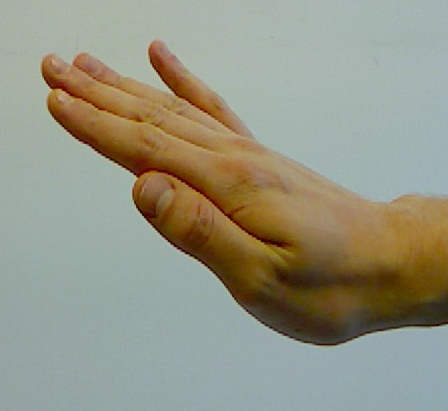
\includegraphics[width=0.2\linewidth,height=0.15\linewidth]{figures/examples/3.jpg}}
\hspace{0.03\linewidth}
\subfloat[Mi]{\label{fig:hand_4}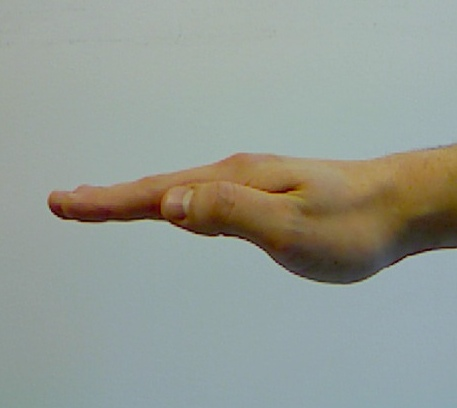
\includegraphics[width=0.2\linewidth,height=0.15\linewidth]{figures/examples/4.jpg}}
\hspace{0.03\linewidth}
\subfloat[Fa]{\label{fig:hand_5}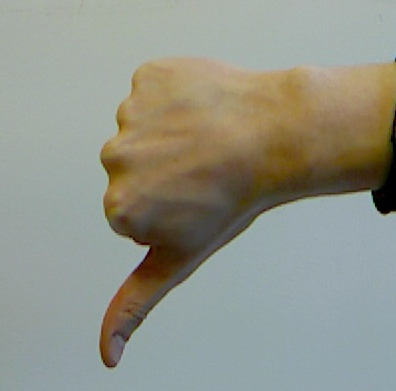
\includegraphics[width=0.2\linewidth,height=0.15\linewidth]{figures/examples/5.jpg}}
\hspace{0.03\linewidth}
\subfloat[Fi]{\label{fig:hand_6}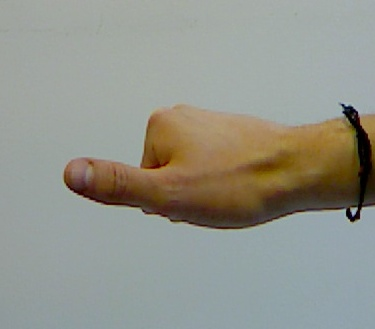
\includegraphics[width=0.2\linewidth,height=0.15\linewidth]{figures/examples/6.jpg}}
\hspace{0.03\linewidth}
\subfloat[Sol]{\label{fig:hand_7}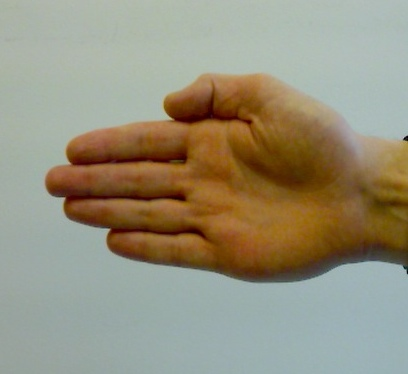
\includegraphics[width=0.2\linewidth,height=0.15\linewidth]{figures/examples/7.jpg}}
\hspace{0.03\linewidth}
\subfloat[Si]{\label{fig:hand_8}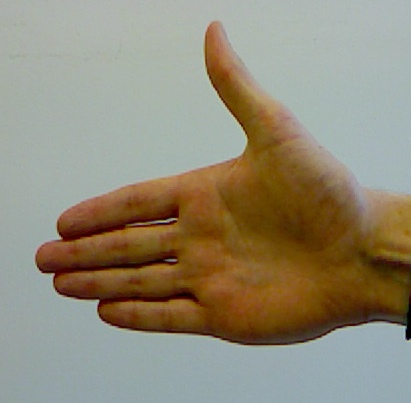
\includegraphics[width=0.2\linewidth,height=0.15\linewidth]{figures/examples/8.jpg}}
\hspace{0.03\linewidth}
\subfloat[La]{\label{fig:hand_9}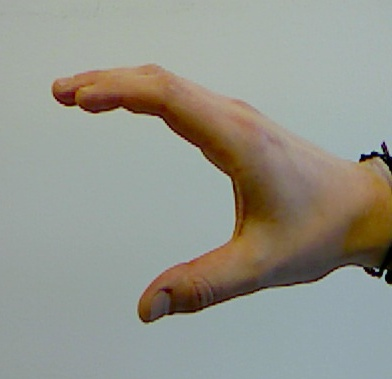
\includegraphics[width=0.2\linewidth,height=0.15\linewidth]{figures/examples/9.jpg}}
\hspace{0.03\linewidth}
\subfloat[Li]{\label{fig:hand_10}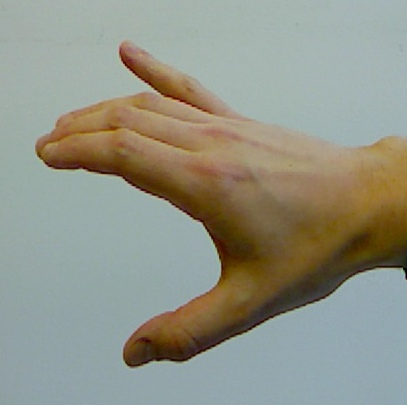
\includegraphics[width=0.2\linewidth,height=0.15\linewidth]{figures/examples/10.jpg}}
\hspace{0.03\linewidth}
\subfloat[Ti]{\label{fig:hand_11}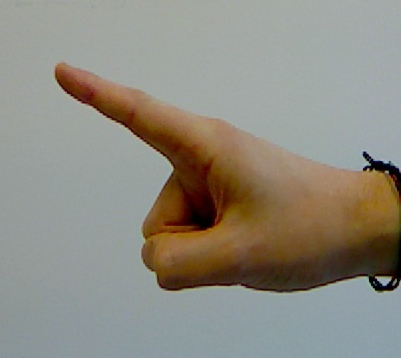
\includegraphics[width=0.2\linewidth,height=0.15\linewidth]{figures/examples/11.jpg}}
\end{center}
\caption{All mirrored Curwen hand poses}
\label{fig:hands_mirrored}
\end{figure}

\begin{figure}[htbp]
\begin{center}
\subfloat[Do]{\label{fig:hand_12}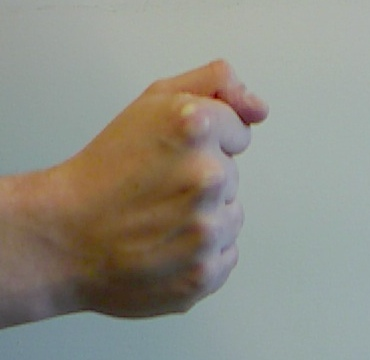
\includegraphics[width=0.2\linewidth,height=0.15\linewidth]{figures/examples/12.jpg}}
\hspace{0.03\linewidth}
\subfloat[Di]{\label{fig:hand_13}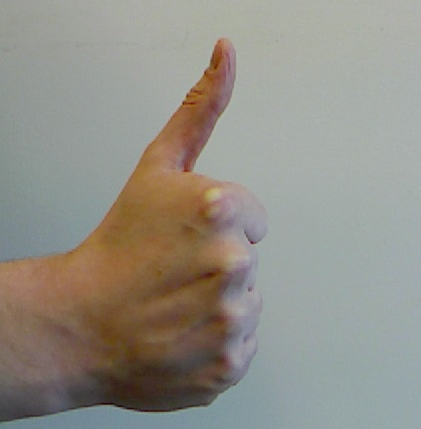
\includegraphics[width=0.2\linewidth,height=0.15\linewidth]{figures/examples/13.jpg}}
\hspace{0.03\linewidth}
\subfloat[Re]{\label{fig:hand_14}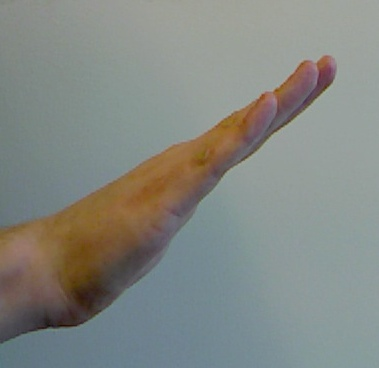
\includegraphics[width=0.2\linewidth,height=0.15\linewidth]{figures/examples/14.jpg}}
\hspace{0.03\linewidth}
\subfloat[Ri]{\label{fig:hand_15}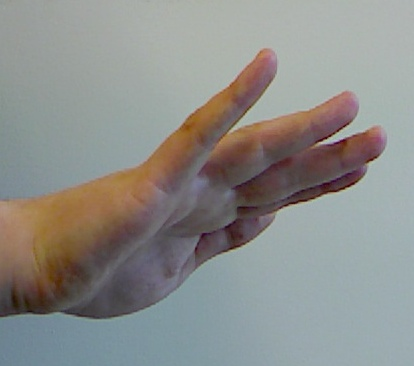
\includegraphics[width=0.2\linewidth,height=0.15\linewidth]{figures/examples/15.jpg}}
\hspace{0.03\linewidth}
\subfloat[Mi]{\label{fig:hand_16}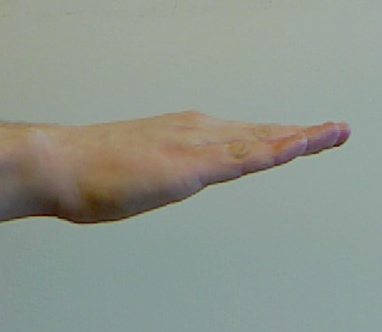
\includegraphics[width=0.2\linewidth,height=0.15\linewidth]{figures/examples/16.jpg}}
\hspace{0.03\linewidth}
\subfloat[Fa]{\label{fig:hand_17}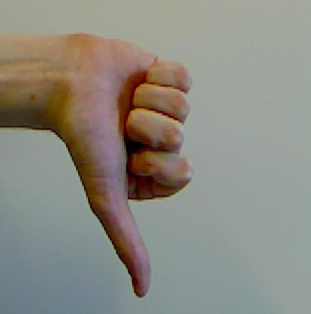
\includegraphics[width=0.2\linewidth,height=0.15\linewidth]{figures/examples/17.jpg}}
\hspace{0.03\linewidth}
\subfloat[Fi]{\label{fig:hand_18}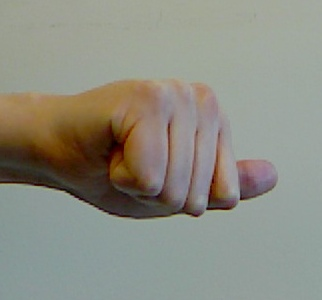
\includegraphics[width=0.2\linewidth,height=0.15\linewidth]{figures/examples/18.jpg}}
\hspace{0.03\linewidth}
\subfloat[Sol]{\label{fig:hand_19}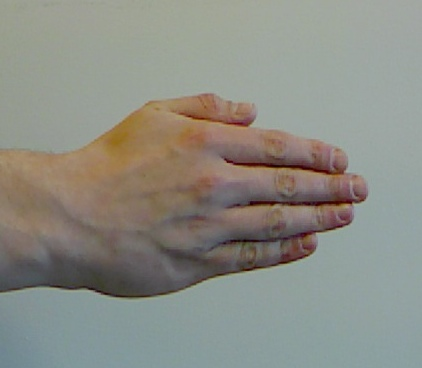
\includegraphics[width=0.2\linewidth,height=0.15\linewidth]{figures/examples/19.jpg}}
\hspace{0.03\linewidth}
\subfloat[Si]{\label{fig:hand_20}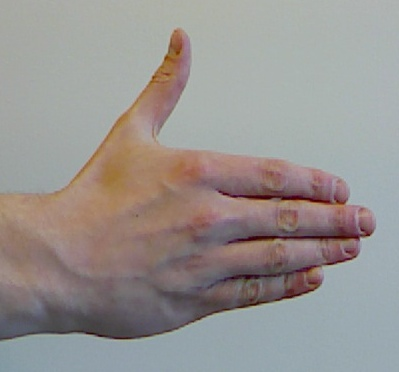
\includegraphics[width=0.2\linewidth,height=0.15\linewidth]{figures/examples/20.jpg}}
\hspace{0.03\linewidth}
\subfloat[La]{\label{fig:hand_21}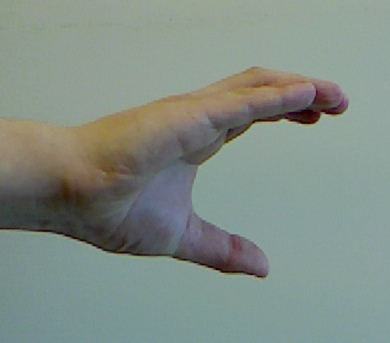
\includegraphics[width=0.2\linewidth,height=0.15\linewidth]{figures/examples/21.jpg}}
\hspace{0.03\linewidth}
\subfloat[Li]{\label{fig:hand_22}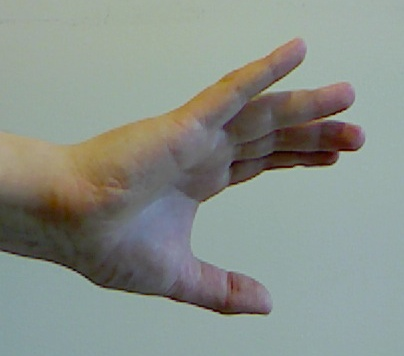
\includegraphics[width=0.2\linewidth,height=0.15\linewidth]{figures/examples/22.jpg}}
\hspace{0.03\linewidth}
\subfloat[Ti]{\label{fig:hand_23}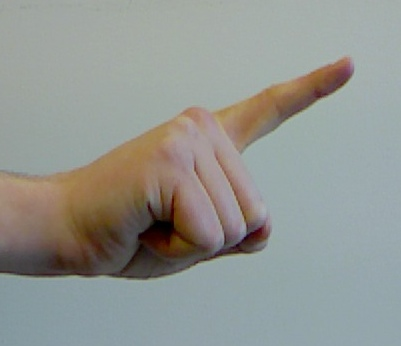
\includegraphics[width=0.2\linewidth,height=0.15\linewidth]{figures/examples/23.jpg}}
\end{center}
\caption{All Curwen hand poses}
\label{fig:hands_normal}
\end{figure}


\begin{figure}[htbp]
\begin{center}
\subfloat[Extra1]{\label{fig:hand_24}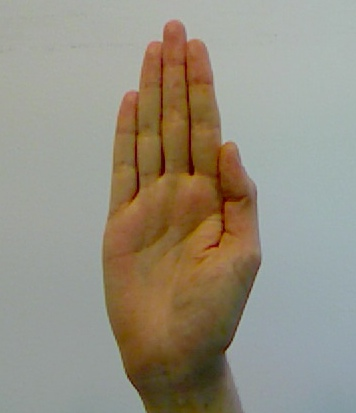
\includegraphics[width=0.2\linewidth,height=0.15\linewidth]{figures/examples/24.jpg}}
\hspace{0.03\linewidth}
\subfloat[Extra2]{\label{fig:hand_25}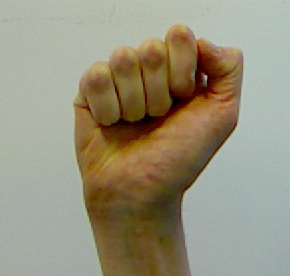
\includegraphics[width=0.2\linewidth,height=0.15\linewidth]{figures/examples/25.jpg}}
\hspace{0.03\linewidth}
\subfloat[Extra3]{\label{fig:hand_26}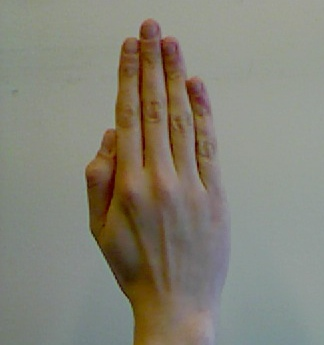
\includegraphics[width=0.2\linewidth,height=0.15\linewidth]{figures/examples/26.jpg}}
\hspace{0.03\linewidth}
\subfloat[Extra4]{\label{fig:hand_27}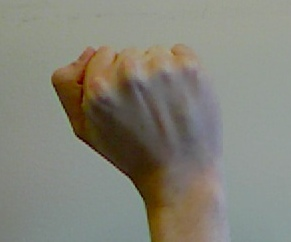
\includegraphics[width=0.2\linewidth,height=0.15\linewidth]{figures/examples/27.jpg}}
\end{center}
\caption{The extra hand poses}
\label{fig:hands_extra}
\end{figure}


\begin{figure}[htbp]
\begin{center}
\subfloat[Do]{\label{fig:gijs5_0}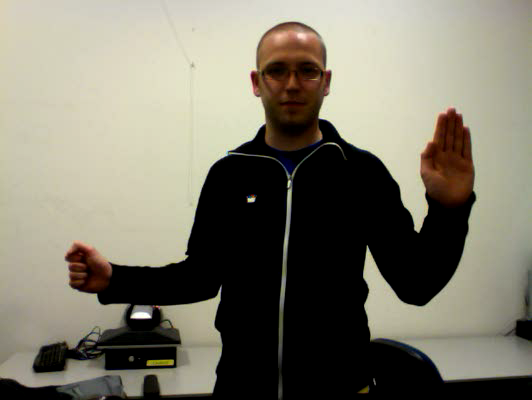
\includegraphics[width=0.2\linewidth,height=0.15\linewidth]{figures/gijs5/0.png}}
\hspace{0.03\linewidth}
\subfloat[Di]{\label{fig:gijs5_1}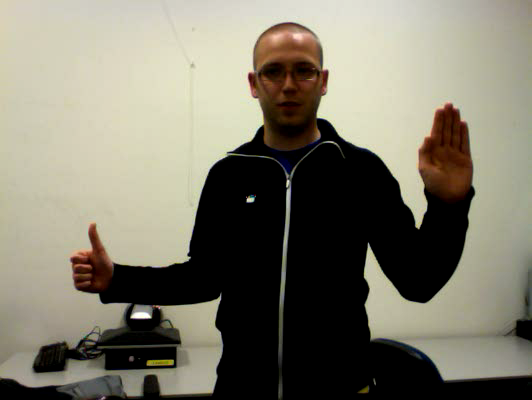
\includegraphics[width=0.2\linewidth,height=0.15\linewidth]{figures/gijs5/1.png}}
\hspace{0.03\linewidth}
\subfloat[Re]{\label{fig:gijs5_2}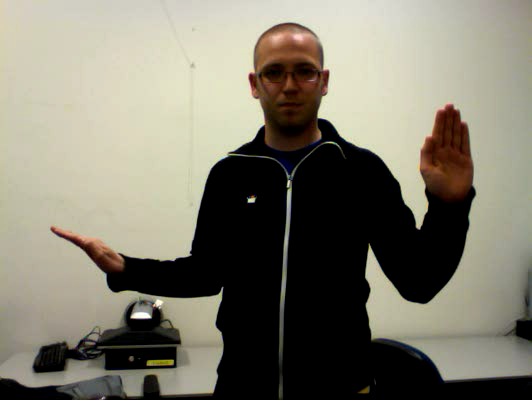
\includegraphics[width=0.2\linewidth,height=0.15\linewidth]{figures/gijs5/2.png}}
\hspace{0.03\linewidth}
\subfloat[Ri]{\label{fig:gijs5_3}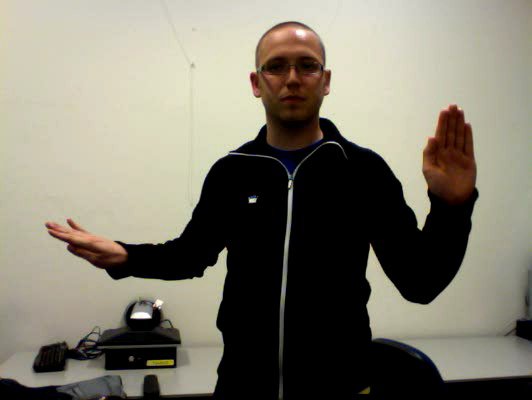
\includegraphics[width=0.2\linewidth,height=0.15\linewidth]{figures/gijs5/3.png}}
\hspace{0.03\linewidth}
\subfloat[Mi]{\label{fig:gijs5_4}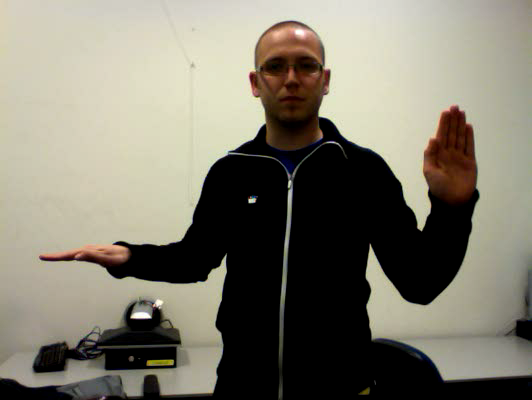
\includegraphics[width=0.2\linewidth,height=0.15\linewidth]{figures/gijs5/4.png}}
\hspace{0.03\linewidth}
\subfloat[Fa]{\label{fig:gijs5_5}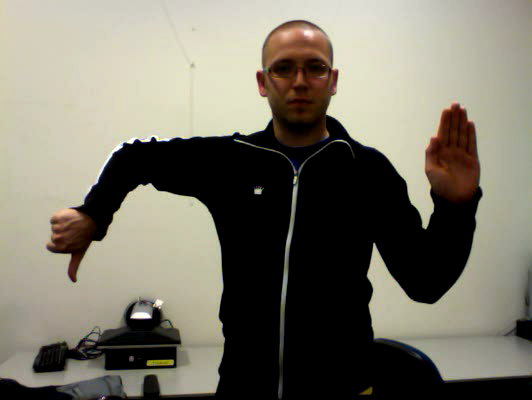
\includegraphics[width=0.2\linewidth,height=0.15\linewidth]{figures/gijs5/5.png}}
\hspace{0.03\linewidth}
\subfloat[Fi]{\label{fig:gijs5_6}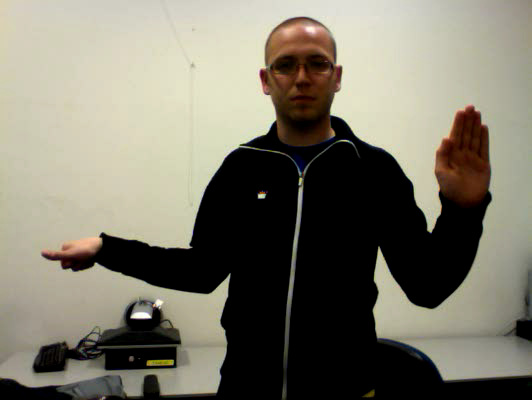
\includegraphics[width=0.2\linewidth,height=0.15\linewidth]{figures/gijs5/6.png}}
\hspace{0.03\linewidth}
\subfloat[Sol]{\label{fig:gijs5_7}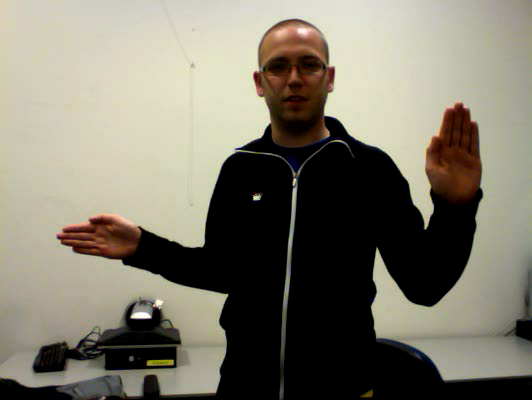
\includegraphics[width=0.2\linewidth,height=0.15\linewidth]{figures/gijs5/7.png}}
\hspace{0.03\linewidth}
\subfloat[Si]{\label{fig:gijs5_8}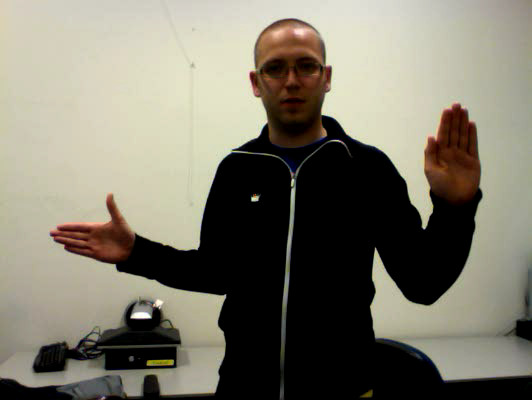
\includegraphics[width=0.2\linewidth,height=0.15\linewidth]{figures/gijs5/8.png}}
\hspace{0.03\linewidth}
\subfloat[La]{\label{fig:gijs5_9}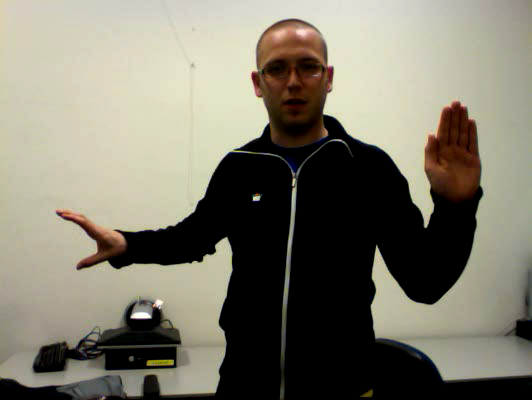
\includegraphics[width=0.2\linewidth,height=0.15\linewidth]{figures/gijs5/9.png}}
\hspace{0.03\linewidth}
\subfloat[Li]{\label{fig:gijs5_10}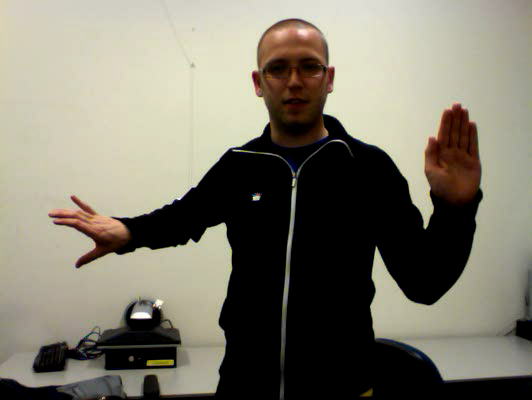
\includegraphics[width=0.2\linewidth,height=0.15\linewidth]{figures/gijs5/10.png}}
\hspace{0.03\linewidth}
\subfloat[Ti]{\label{fig:gijs5_11}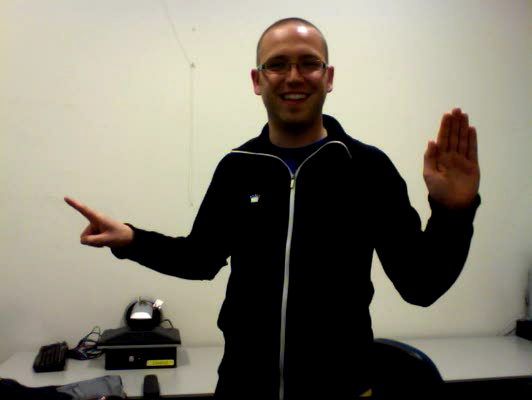
\includegraphics[width=0.2\linewidth,height=0.15\linewidth]{figures/gijs5/11.png}}
\hspace{0.03\linewidth}
\subfloat[Do]{\label{fig:gijs5_12}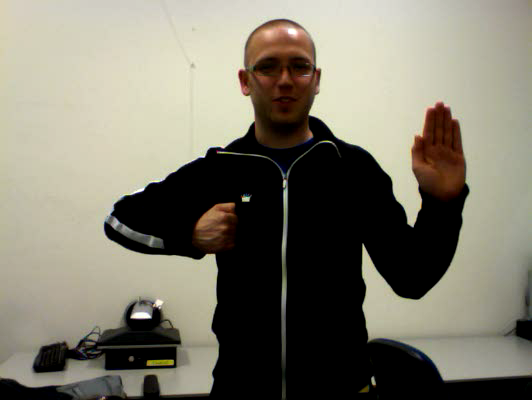
\includegraphics[width=0.2\linewidth,height=0.15\linewidth]{figures/gijs5/12.png}}
\hspace{0.03\linewidth}
\subfloat[Di]{\label{fig:gijs5_13}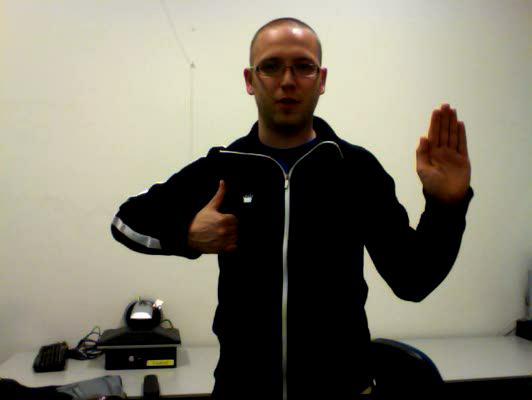
\includegraphics[width=0.2\linewidth,height=0.15\linewidth]{figures/gijs5/13.png}}
\hspace{0.03\linewidth}
\subfloat[Re]{\label{fig:gijs5_14}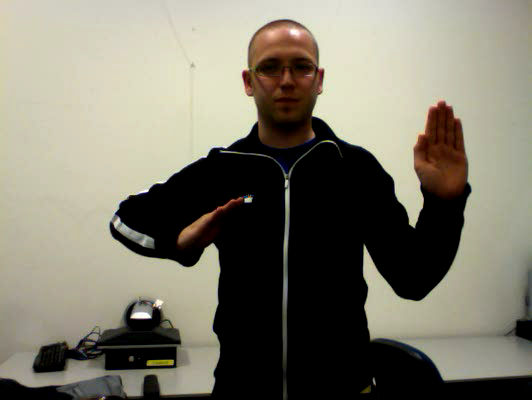
\includegraphics[width=0.2\linewidth,height=0.15\linewidth]{figures/gijs5/14.png}}
\hspace{0.03\linewidth}
\subfloat[Ri]{\label{fig:gijs5_15}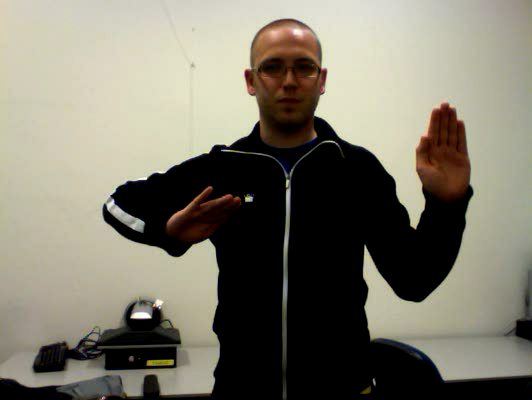
\includegraphics[width=0.2\linewidth,height=0.15\linewidth]{figures/gijs5/15.png}}
\hspace{0.03\linewidth}
\subfloat[Mi]{\label{fig:gijs5_16}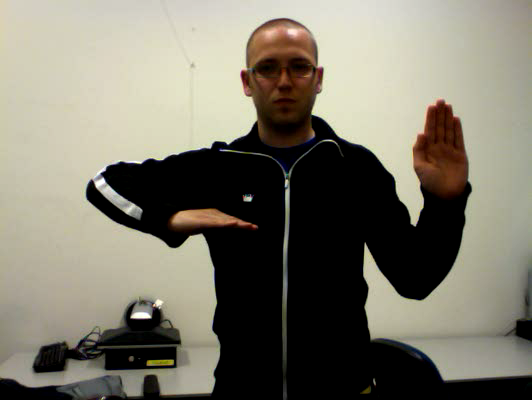
\includegraphics[width=0.2\linewidth,height=0.15\linewidth]{figures/gijs5/16.png}}
\hspace{0.03\linewidth}
\subfloat[Fa]{\label{fig:gijs5_17}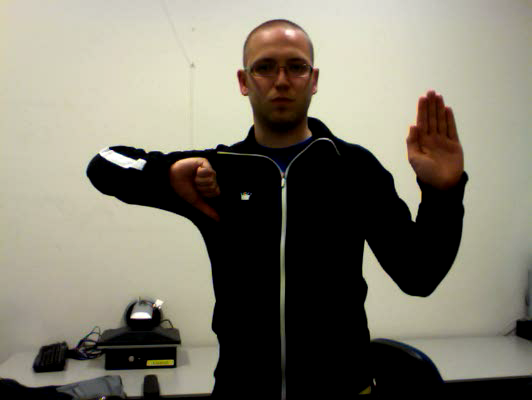
\includegraphics[width=0.2\linewidth,height=0.15\linewidth]{figures/gijs5/17.png}}
\hspace{0.03\linewidth}
\subfloat[Fi]{\label{fig:gijs5_18}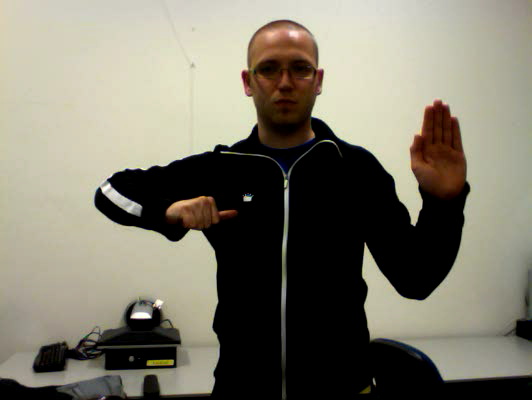
\includegraphics[width=0.2\linewidth,height=0.15\linewidth]{figures/gijs5/18.png}}
\hspace{0.03\linewidth}
\subfloat[Sol]{\label{fig:gijs5_19}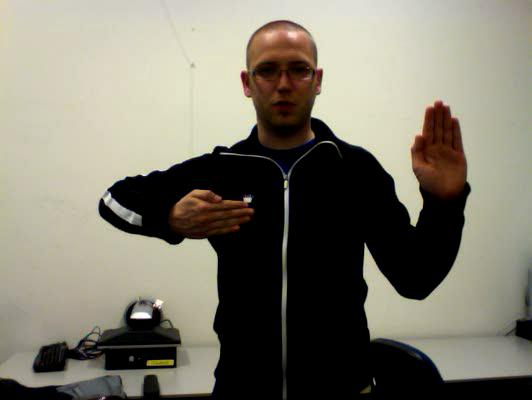
\includegraphics[width=0.2\linewidth,height=0.15\linewidth]{figures/gijs5/19.png}}
\hspace{0.03\linewidth}
\subfloat[Si]{\label{fig:gijs5_20}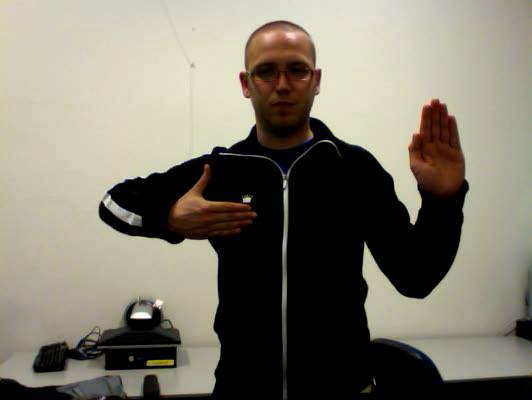
\includegraphics[width=0.2\linewidth,height=0.15\linewidth]{figures/gijs5/20.png}}
\hspace{0.03\linewidth}
\subfloat[La]{\label{fig:gijs5_21}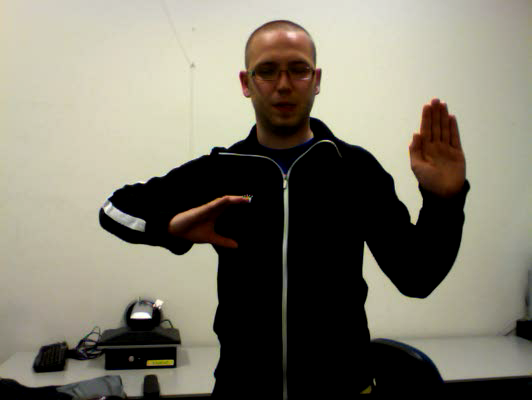
\includegraphics[width=0.2\linewidth,height=0.15\linewidth]{figures/gijs5/21.png}}
\hspace{0.03\linewidth}
\subfloat[Li]{\label{fig:gijs5_22}\includegraphics[width=0.2\linewidth,height=0.15\linewidth]{figures/gijs5/22.png}}
\hspace{0.03\linewidth}
\subfloat[Ti]{\label{fig:gijs5_23}\includegraphics[width=0.2\linewidth,height=0.15\linewidth]{figures/gijs5/23.png}}
\hspace{0.03\linewidth}
\subfloat[Extra1]{\label{fig:gijs5_24}\includegraphics[width=0.2\linewidth,height=0.15\linewidth]{figures/gijs5/24.png}}
\hspace{0.03\linewidth}
\subfloat[Extra2]{\label{fig:gijs5_25}\includegraphics[width=0.2\linewidth,height=0.15\linewidth]{figures/gijs5/25.png}}
\hspace{0.03\linewidth}
\subfloat[Extra3]{\label{fig:gijs5_26}\includegraphics[width=0.2\linewidth,height=0.15\linewidth]{figures/gijs5/26.png}}
\hspace{0.03\linewidth}
\subfloat[Extra4]{\label{fig:gijs5_27}\includegraphics[width=0.2\linewidth,height=0.15\linewidth]{figures/gijs5/27.png}}
\end{center}
\caption{Stills from recording number 5, test subject 'gijs'}
\label{fig:gijs5}
\end{figure}



\begin{figure}[htbp]
\begin{center}
\subfloat[Do]{\label{fig:gijs5_cutout_0}\includegraphics[width=0.2\linewidth,height=0.15\linewidth]{figures/gijs5_cutout/0.jpg}}
\hspace{0.03\linewidth}
\subfloat[Di]{\label{fig:gijs5_cutout_1}\includegraphics[width=0.2\linewidth,height=0.15\linewidth]{figures/gijs5_cutout/1.jpg}}
\hspace{0.03\linewidth}
\subfloat[Re]{\label{fig:gijs5_cutout_2}\includegraphics[width=0.2\linewidth,height=0.15\linewidth]{figures/gijs5_cutout/2.jpg}}
\hspace{0.03\linewidth}
\subfloat[Ri]{\label{fig:gijs5_cutout_3}\includegraphics[width=0.2\linewidth,height=0.15\linewidth]{figures/gijs5_cutout/3.jpg}}
\hspace{0.03\linewidth}
\subfloat[Mi]{\label{fig:gijs5_cutout_4}\includegraphics[width=0.2\linewidth,height=0.15\linewidth]{figures/gijs5_cutout/4.jpg}}
\hspace{0.03\linewidth}
\subfloat[Fa]{\label{fig:gijs5_cutout_5}\includegraphics[width=0.2\linewidth,height=0.15\linewidth]{figures/gijs5_cutout/5.jpg}}
\hspace{0.03\linewidth}
\subfloat[Fi]{\label{fig:gijs5_cutout_6}\includegraphics[width=0.2\linewidth,height=0.15\linewidth]{figures/gijs5_cutout/6.jpg}}
\hspace{0.03\linewidth}
\subfloat[Sol]{\label{fig:gijs5_cutout_7}\includegraphics[width=0.2\linewidth,height=0.15\linewidth]{figures/gijs5_cutout/7.jpg}}
\hspace{0.03\linewidth}
\subfloat[Si]{\label{fig:gijs5_cutout_8}\includegraphics[width=0.2\linewidth,height=0.15\linewidth]{figures/gijs5_cutout/8.jpg}}
\hspace{0.03\linewidth}
\subfloat[La]{\label{fig:gijs5_cutout_9}\includegraphics[width=0.2\linewidth,height=0.15\linewidth]{figures/gijs5_cutout/9.jpg}}
\hspace{0.03\linewidth}
\subfloat[Li]{\label{fig:gijs5_cutout_10}\includegraphics[width=0.2\linewidth,height=0.15\linewidth]{figures/gijs5_cutout/10.jpg}}
\hspace{0.03\linewidth}
\subfloat[Ti]{\label{fig:gijs5_cutout_11}\includegraphics[width=0.2\linewidth,height=0.15\linewidth]{figures/gijs5_cutout/11.jpg}}
\hspace{0.03\linewidth}
\subfloat[Do]{\label{fig:gijs5_cutout_12}\includegraphics[width=0.2\linewidth,height=0.15\linewidth]{figures/gijs5_cutout/12.jpg}}
\hspace{0.03\linewidth}
\subfloat[Di]{\label{fig:gijs5_cutout_13}\includegraphics[width=0.2\linewidth,height=0.15\linewidth]{figures/gijs5_cutout/13.jpg}}
\hspace{0.03\linewidth}
\subfloat[Re]{\label{fig:gijs5_cutout_14}\includegraphics[width=0.2\linewidth,height=0.15\linewidth]{figures/gijs5_cutout/14.jpg}}
\hspace{0.03\linewidth}
\subfloat[Ri]{\label{fig:gijs5_cutout_15}\includegraphics[width=0.2\linewidth,height=0.15\linewidth]{figures/gijs5_cutout/15.jpg}}
\hspace{0.03\linewidth}
\subfloat[Mi]{\label{fig:gijs5_cutout_16}\includegraphics[width=0.2\linewidth,height=0.15\linewidth]{figures/gijs5_cutout/16.jpg}}
\hspace{0.03\linewidth}
\subfloat[Fa]{\label{fig:gijs5_cutout_17}\includegraphics[width=0.2\linewidth,height=0.15\linewidth]{figures/gijs5_cutout/17.jpg}}
\hspace{0.03\linewidth}
\subfloat[Fi]{\label{fig:gijs5_cutout_18}\includegraphics[width=0.2\linewidth,height=0.15\linewidth]{figures/gijs5_cutout/18.jpg}}
\hspace{0.03\linewidth}
\subfloat[Sol]{\label{fig:gijs5_cutout_19}\includegraphics[width=0.2\linewidth,height=0.15\linewidth]{figures/gijs5_cutout/19.jpg}}
\hspace{0.03\linewidth}
\subfloat[Si]{\label{fig:gijs5_cutout_20}\includegraphics[width=0.2\linewidth,height=0.15\linewidth]{figures/gijs5_cutout/20.jpg}}
\hspace{0.03\linewidth}
\subfloat[La]{\label{fig:gijs5_cutout_21}\includegraphics[width=0.2\linewidth,height=0.15\linewidth]{figures/gijs5_cutout/21.jpg}}
\hspace{0.03\linewidth}
\subfloat[Li]{\label{fig:gijs5_cutout_22}\includegraphics[width=0.2\linewidth,height=0.15\linewidth]{figures/gijs5_cutout/22.jpg}}
\hspace{0.03\linewidth}
\subfloat[Ti]{\label{fig:gijs5_cutout_23}\includegraphics[width=0.2\linewidth,height=0.15\linewidth]{figures/gijs5_cutout/23.jpg}}
\hspace{0.03\linewidth}
\subfloat[Extra1]{\label{fig:gijs5_cutout_24}\includegraphics[width=0.2\linewidth,height=0.15\linewidth]{figures/gijs5_cutout/24.jpg}}
\hspace{0.03\linewidth}
\subfloat[Extra2]{\label{fig:gijs5_cutout_25}\includegraphics[width=0.2\linewidth,height=0.15\linewidth]{figures/gijs5_cutout/25.jpg}}
\hspace{0.03\linewidth}
\subfloat[Extra3]{\label{fig:gijs5_cutout_26}\includegraphics[width=0.2\linewidth,height=0.15\linewidth]{figures/gijs5_cutout/26.jpg}}
\hspace{0.03\linewidth}
\subfloat[Extra4]{\label{fig:gijs5_cutout_27}\includegraphics[width=0.2\linewidth,height=0.15\linewidth]{figures/gijs5_cutout/27.jpg}}
\end{center}
\caption{Cutout hands, test subject 'gijs' recording number 5}
\label{fig:gijs5_cutout}
\end{figure}



